\documentclass[gray]{beamer}

\usefonttheme{serif}
\setbeamerfont{title}{series=\bfseries,parent=structure}
\setbeamerfont{frametitle}{series=\bfseries,parent=structure}
\setbeamertemplate{itemize items}[circle]

\setbeamertemplate{footline}
{
  \hbox{\begin{beamercolorbox}[wd=1\paperwidth,ht=2.25ex,dp=1ex,right]{framenumber}%
      \usebeamerfont{framenumber}\insertframenumber{} / \inserttotalframenumber\hspace*{2ex}
    \end{beamercolorbox}}%
  \vskip0pt%
}

\beamertemplatenavigationsymbolsempty

\usepackage[utf8]{inputenc}
\usepackage[T1]{fontenc}
\usepackage{amsthm,amsmath,amsfonts}

\title{Probit Regression for Large Data Sets via Coresets}
\author{Alexander Munteanu \and Simon Omlor \and Christian Peters}
\institute{TU Dortmund University, Germany}
\date{December 18, 2021}

\begin{document}

\begin{frame}[noframenumbering]
    \thispagestyle{empty}
    \maketitle
\end{frame}

\begin{frame}{Probit Regression} \pause
    \textbf{Data:}
    \begin{itemize}
        \item $n$ observations: $x_1, \ldots, x_n \in \mathbb{R}^d$ \\
        \item with $n$ labels: $y_1, \ldots, y_n \in \{-1, 1\}$
    \end{itemize}

    \pause

    \vspace{\fill}

    \textbf{Model:}
    \begin{itemize}
        \item $y_1, \ldots, y_n$ are realizations of $Y_1, \ldots, Y_n$
        \item $Y_i \sim Bin(1, \pi_i), \quad \pi_i = \Phi(x_i^T \beta)$
        \item $\Phi(\cdot)$ is cdf of standard normal distribution
    \end{itemize}

    \pause

    \vspace{\fill}

    \textbf{Loss function (negative log-likelihood):}
    \begin{equation*}
        f(\beta) = \sum_{i=1}^n \ln\left( \frac{1}{\Phi(y_ix_i^T\beta)} \right)
    \end{equation*}
\end{frame}

\begin{frame}{The Problem} \pause
    \textbf{Problems with large datasets:}
    \begin{itemize}
        \item Data doesn't fit into main memory
        \item Limited access to the data (e.g. data streams)
    \end{itemize}

    \pause

    \vspace{\fill}

    \textbf{Scenarios where this can happen:%
        \footnote<.(1)->{see e.g. \cite{big-data-tiny-data}}}
    \begin{itemize}
        \item Sensor data from mobile devices, cameras, ...
        \item Internet logs
        \item Financial data
    \end{itemize}

    \pause

    \vspace{\fill}

    \textbf{$\Rightarrow$ Conventional optimization algorithms become inefficient!}
\end{frame}

\begin{frame}{Our Solution} \pause
    \textbf{Select only a small subset (coreset) of the data!} \\
    $\Rightarrow$ Fit the model on the coreset.

    \pause

    \vspace{\fill}

    \textbf{Challenges:}
    \begin{itemize}
        \item Results on coreset must be close to results on original data
              \begin{itemize}
                  \item[$\Rightarrow$] Need theoretical guarantees!
              \end{itemize}
        \item Coreset must be significantly smaller than original data
              \begin{itemize}
                  \item[$\Rightarrow$] Otherwise useless!
              \end{itemize}
    \end{itemize}

    \pause

    \vspace{\fill}

    \textbf{Main Goal: Develop efficient coreset construction algorithms!}
\end{frame}

\begin{frame}{The coresets we want...} \pause
    \textbf{(1) ...approximate the data well:}
    \begin{itemize}
        \item Let $f(\beta)$ be the original loss and $\tilde{f}(\beta)$
              be the loss on the coreset
        \item Then for $\epsilon > 0$ and for all $\beta \in \mathbb{R}^d$ we want:
              \begin{equation*}
                  (1 - \epsilon) f(\beta) \leq \tilde{f}(\beta) \leq (1 + \epsilon) f(\beta)
              \end{equation*}
        \item This criterion will guarantee our approximation quality!
    \end{itemize}

    \pause

    \vspace{\fill}

    \textbf{(2) ...are significantly smaller than our data:}
    \begin{itemize}
        \item Coreset sizes logarithmic in $n$ would be a great success
        \item Given a dataset with $n=1,000,000,000$ observations,
              $\log(n) \leq 21$
        \item Even better: Independent of $n$!
    \end{itemize}
\end{frame}

\begin{frame}{Our first obstacle} \pause
    \textbf{Not every data set allows for small coresets.}
    \begin{itemize}
        \item Shown in \cite{on-coresets} for logistic regression,
              but proof is similar for probit regression
    \end{itemize}

    \pause

    \vspace{\fill}

    \textbf{$\Rightarrow$ Need to restrict the class of data sets under study!}
    \begin{itemize}
        \item Slightly adapt the concept of $\mu$-complexity from
              \cite{on-coresets} to probit regression
    \end{itemize}
\end{frame}

\begin{frame}{$\mu$-Complexity} \pause
    $\mu$ is a useful parameter introduced by \cite{on-coresets}:
    \begin{equation*}
        \mu = \sup_{\beta \in \mathbb{R}^d \setminus \{0\} }
        \frac{\sum_{y_ix_i^T\beta > 0} (x_i^T \beta)^2}
        {\sum_{y_ix_i^T\beta < 0}(x_i^T \beta)^2}
    \end{equation*}

    \pause

    \vspace{\fill}

    Finite $\mu$, i.e. $\mu$-complexity ensures:
    \begin{itemize}
        \item That the data is not linearly separable
        \item That the optimum of the loss function exists and is unqiue
    \end{itemize}

    \pause

    \vspace{\fill}

    \textbf{We show how $\mu$ can be used to find small coresets!}
\end{frame}

\begin{frame}{How to tackle coreset construction?} \pause
    \textbf{Idea: Use random sampling of observations!}

    \pause

    \vspace{\fill}

    \textbf{Problem: Which sampling distribution to use?}
    \begin{itemize}
        \item Uniform equal probability sampling is not a good idea
        \item It is known to fail when the data has outliers
        \item[$\Rightarrow$] We need to give "important" observations a
              higher priority
    \end{itemize}

    \pause

    \vspace{\fill}

    \textbf{Our approach: Use importance sampling based on the
        sensitivity\footnote<.(1)->{see \cite{langberg-schulman-sensitivities}} of each observation!}
\end{frame}

\begin{frame}{The Sensitivity Framework}\pause

    \begin{itemize}
        \item Well known algorithmic framework for coreset construction via
              importance sampling introduced by \cite{feldman-langberg-coresets}.
        \item The sensitivity is the worst-case importance of an observation
        \item Sampling proportionally to upper bounds on the sensitivities
              can lead to small coresets
        \item[$\Rightarrow$] Need to derive tight upper bounds!
    \end{itemize}

    \pause

    \vspace{\fill}

    \textbf{We show that the statistical leverage scores can be
        used to bound the sensitivities!}

\end{frame}

\begin{frame}{Statistical Leverage Scores}
    \begin{figure}[ht!]
        \centering
        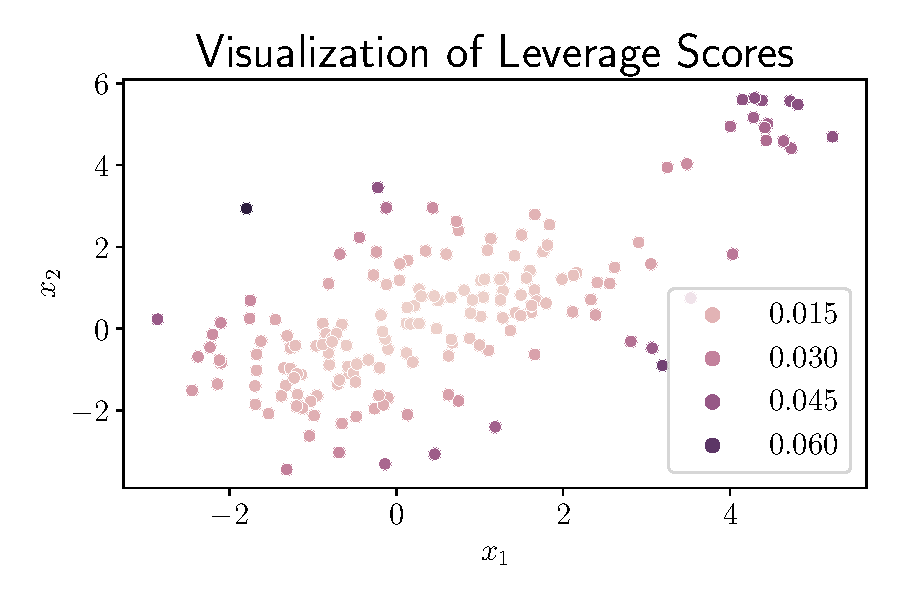
\includegraphics[width=\linewidth]{../figures/leverage_scores_visualization.pdf}
    \end{figure}
\end{frame}

\begin{frame}{First Algorithm: Fast Leverage Score Sampling}\pause
    \textbf{First pass: Approximate the leverage scores}
    \begin{itemize}
        \item Use sketching techniques by \cite{woodruff-2017} to
              approximate the leverage scores
    \end{itemize}

    \pause

    \vspace{\fill}

    \textbf{Second pass: Draw the random sample}
    \begin{itemize}
        \item Use a reservoir sampler, e.g. by \cite{reservoir-sampler}
    \end{itemize}

    \pause

    \vspace{\fill}

    \centering
    \fbox{\textbf{Coreset size: $O\left(\frac{\mu d^2}{\epsilon^2}\right)$, independent of $n$!}}
\end{frame}

\begin{frame}{Second Algorithm: Online Leverage Score Sampling} \pause
    \textbf{Problem:} First algorithm needs two passes.

    \pause

    \vspace{\fill}

    \textbf{Solution:} Online approximation of the leverage scores
    \begin{itemize}
        \item Use approximation techniques by \cite{tensor-factorization}
        \item Increases coreset size by a factor of $\log(\sigma_{max})$
              \begin{itemize}
                  \item $\sigma_{max}$ is largest singular value of the data matrix
              \end{itemize}
        \item Needs $O(d^2)$ update time
    \end{itemize}

    \pause

    \vspace{\fill}

    \textbf{Requires only one pass over the data set!}
\end{frame}

\begin{frame}{Experiments} \pause
    \textbf{Goal: Compare our algorithms to uniform random sampling}
    \begin{itemize}
        \item Show that coreset construction is worth the effort
    \end{itemize}

    \pause

    \vspace{\fill}

    \textbf{Use approximation ratio for evaluation:}
    \begin{itemize}
        \item Let $\tilde{f}(\beta)$ be the loss function on the coreset
              and let $f(\beta)$ be the original loss
        \item Let $\beta^{opt}$ be the solution of the original problem
        \item Optimize $\tilde{f}(\beta)$ to find solution $\tilde{\beta}$
              of the reduced problem
        \item Compute ratio $\frac{f(\tilde{\beta})}{f(\beta^{opt})}$
    \end{itemize}
\end{frame}

\begin{frame}{Experiments}
    \begin{figure}[ht!]
        \centering
        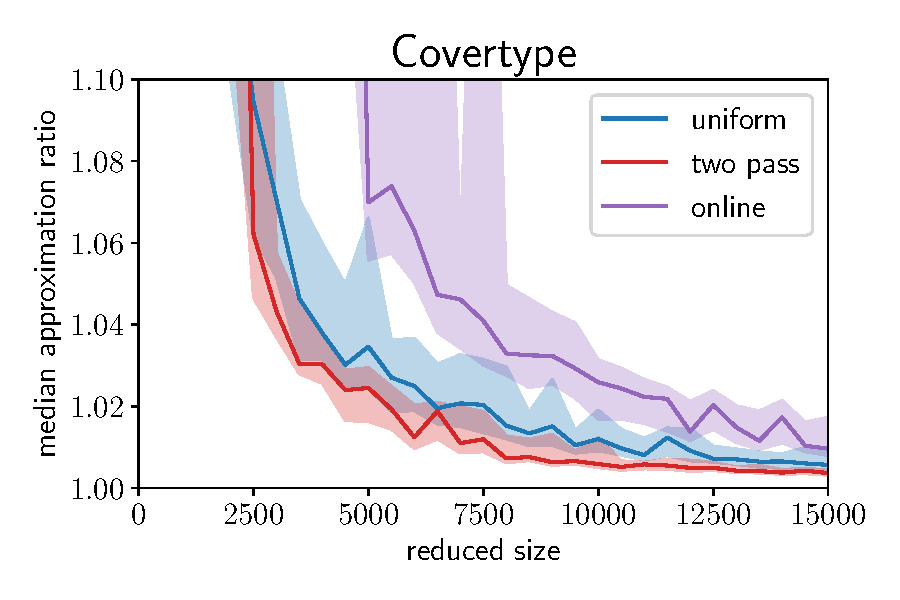
\includegraphics[width=.49\linewidth]{../figures/covertype_ratio_plot.pdf}
        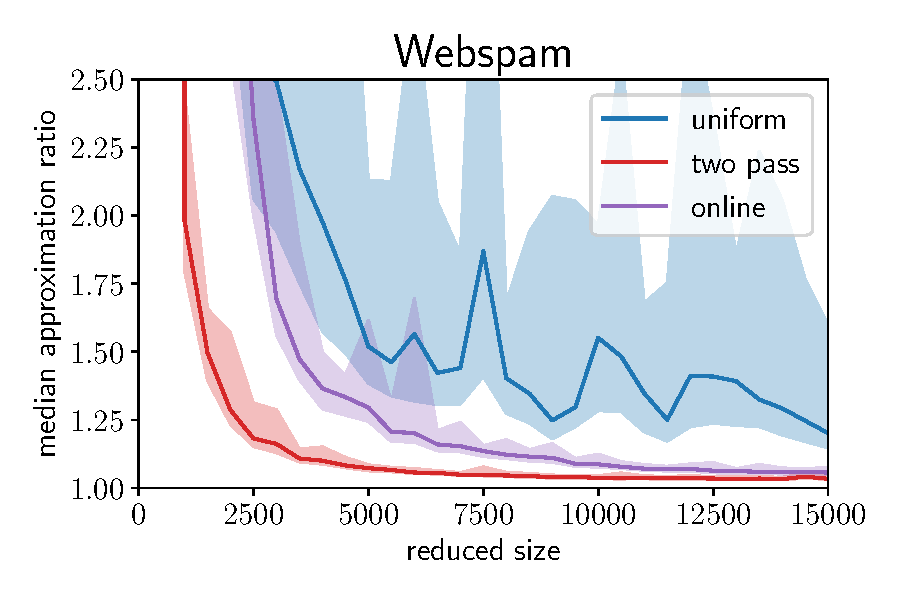
\includegraphics[width=.49\linewidth]{../figures/webspam_ratio_plot.pdf}
        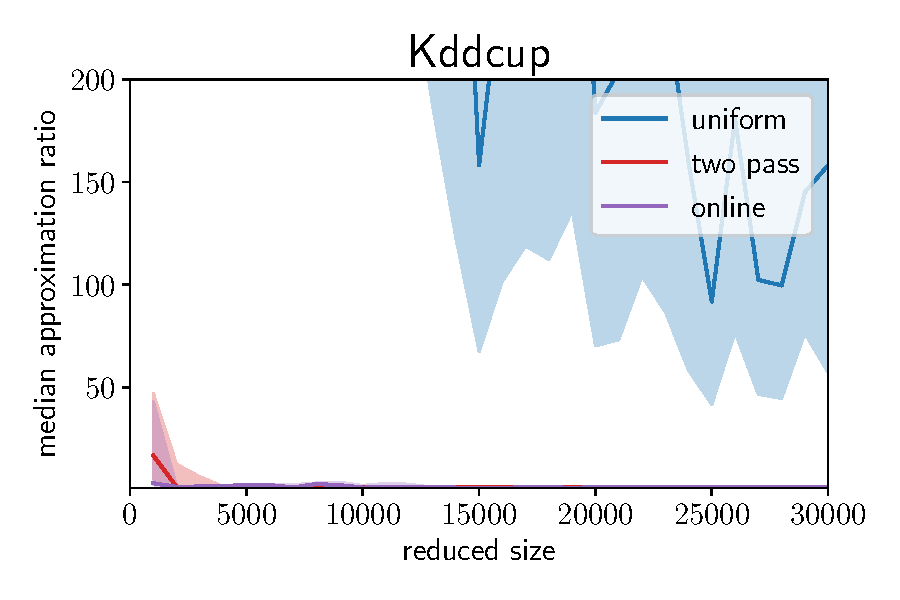
\includegraphics[width=.49\linewidth]{../figures/kddcup_ratio_plot.pdf}
        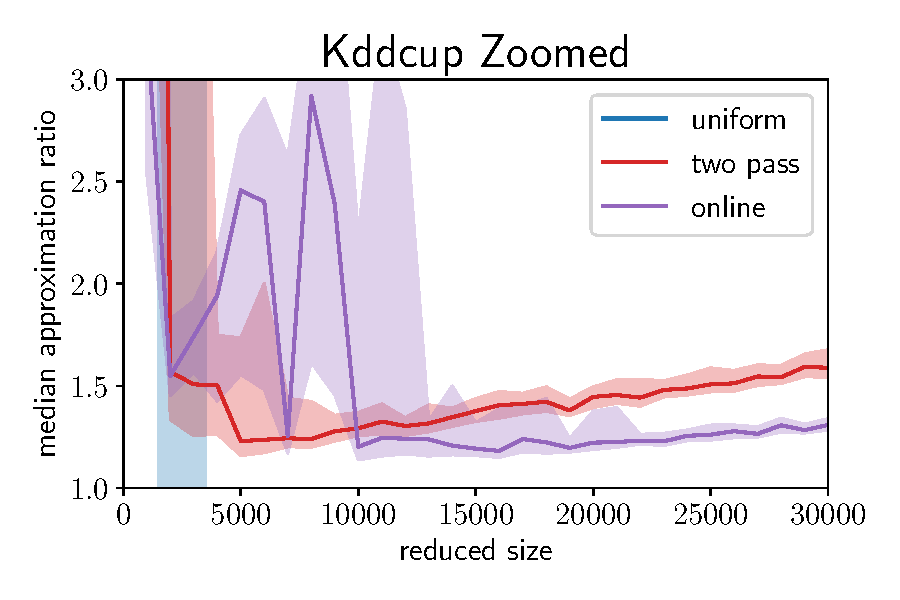
\includegraphics[width=.49\linewidth]{../figures/kddcup_ratio_plot_zoomed.pdf}
    \end{figure}
\end{frame}

\begin{frame}{Extensions -- $p$-Generalized Probit
        Model\footnote{See \cite{KalkeR13} for a definition of the $p$-generalized normal distribution}}
    \begin{figure}[ht!]
        \centering
        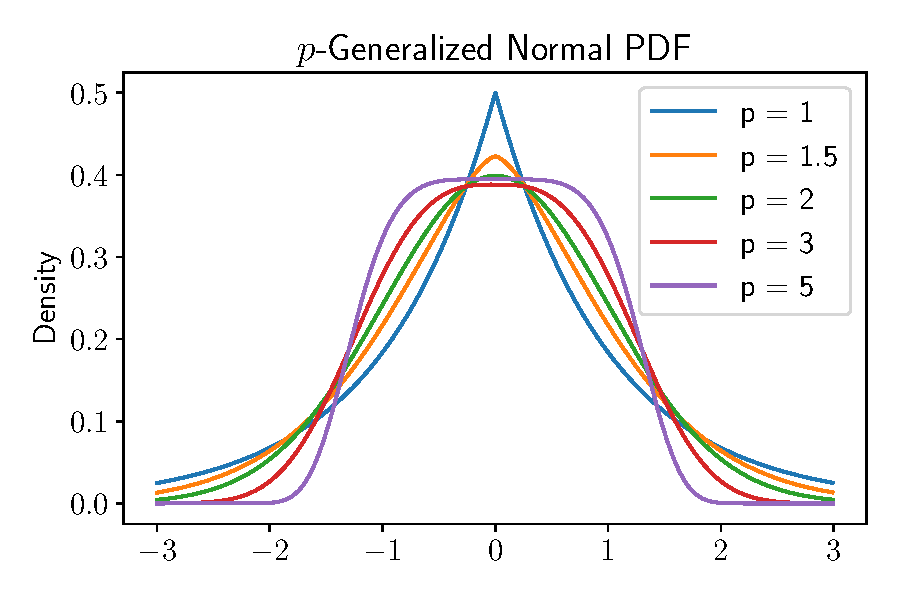
\includegraphics[width=\linewidth]{../figures/p_gen_pdf.pdf}
    \end{figure}
\end{frame}

\begin{frame}{Extensions -- $p$-Generalized Probit Model}
    \textbf{Three adaptations are required:}

    \vspace{\fill}

    \textbf{(1) Need to adapt $\mu$:}
    \begin{equation*}
        \mu = \sup_{\beta \in \mathbb{R}^d \setminus \{0\} }
        \frac{\sum_{y_ix_i^T\beta > 0} |x_i^T \beta|^p}
        {\sum_{y_ix_i^T\beta < 0}|x_i^T \beta|^p}
    \end{equation*}

    \pause

    \vspace{\fill}

    \textbf{(2) Need to use $p$-generalized leverage scores}

    \pause

    \vspace{\fill}

    \textbf{(3) Need to adapt the sketching techniques}

    \pause

    \vspace{\fill}

    \begin{equation*}
        \text{\textbf{Coreset size:} } \begin{cases}
            O\left(\frac{\mu d^p}{\epsilon^2}\right),    & for\ p \in [1, 2)      \\
            O\left(\frac{\mu d^{2p}}{\epsilon^2}\right), & for\ p \in (2, \infty)
        \end{cases}
    \end{equation*}
\end{frame}

\begin{frame}{Recap: Our Contributions} \pause
    \textbf{(1) Enabled scalable maximum likelihood estimation of
        probit models on large datasets}
    \begin{itemize}
        \item Based on fast coreset construction algorithms and modern sketching techniques
    \end{itemize}

    \pause

    \vspace{\fill}

    \textbf{(2) Demonstrated that our methods outperform standard
        uniform sampling}
    \begin{itemize}
        \item By conducting experiments on well known real-world datasets
    \end{itemize}

    \pause

    \vspace{\fill}

    \textbf{(3) Introduced the $p$-generalized probit model as a
        flexible framework for modeling binary data}
    \begin{itemize}
        \item Enables you to control the tail behavior of the distribution
    \end{itemize}
\end{frame}

\setbeamertemplate{footline}{}

\begin{frame}[allowframebreaks, noframenumbering]{Literature}
    % \nocite{*}
    \bibliographystyle{apalike}
    \bibliography{../literature}
\end{frame}

\end{document}
